\documentclass[a4paper,12pt]{article}
\usepackage[utf8]{inputenc}
\usepackage[vietnamese]{babel}
\usepackage{titlesec}
\usepackage{geometry}
\usepackage{graphicx}
\usepackage{fancyhdr}
\usepackage{tocloft}
\usepackage{hyperref}
\usepackage{setspace}
\usepackage{amsmath}
\usepackage{float}
\usepackage[most]{tcolorbox}
\usepackage{tikz}
\usepackage{everypage-1x}
\usepackage{atbegshi}
\usepackage{eso-pic}
\usepackage{enumitem}

\geometry{left=2cm,right=1.5cm,top=2cm,bottom=2.5cm}
\onehalfspacing

\setcounter{secnumdepth}{4}
\setcounter{tocdepth}{4}
\renewcommand{\theparagraph}{\thesubsubsection.\arabic{paragraph}}
\titleformat{\paragraph}[block]{\normalfont\normalsize\bfseries}{\theparagraph}{1em}{}
\titleformat{\section}{\bfseries\large}{\thesection}{1em}{}
\titleformat{\subsection}{\bfseries\normalsize}{\thesubsection}{1em}{}
\renewcommand{\cftsecleader}{\cftdotfill{\cftdotsep}}
\renewcommand{\cftsecfont}{\normalfont}
\renewcommand{\cftsecpagefont}{\normalfont}
\renewcommand{\cfttoctitlefont}{\normalfont\bfseries\Large}
\renewcommand{\cftaftertoctitle}{\hfill}
\renewcommand{\thesection}{\Roman{section}} % Section: La Mã
\renewcommand{\thesubsection}{\arabic{subsection}} % Subsection: 1, 2, 3...
\renewcommand{\thesubsubsection}{\arabic{subsection}.\arabic{subsubsection}} % Subsubsection: 1.1, 2.1,...
% Vẽ khung cho trang bìa
\usepackage{atbegshi}
\AddToShipoutPictureBG*{%
    \ifnum\value{page}=1
    \AtPageLowerLeft{%
        \begin{tikzpicture}[remember picture, overlay]
            \draw[thick, black] 
                ([xshift=1.5cm, yshift=-1.5cm] current page.north west)
                rectangle 
                ([xshift=-1.5cm, yshift=2cm] current page.south east);
        \end{tikzpicture}
    }
}

\hypersetup{
    colorlinks=true, % Bỏ khung đỏ, chỉ hiển thị liên kết màu
    linkcolor=black, % Màu liên kết trong nội dung
    filecolor=black, % Màu liên kết file
    urlcolor=blue, % Màu liên kết URL
    citecolor=black % Màu liên kết trích dẫn
}


\begin{document}
%----------------------------------
% Trang bìa
%----------------------------------
\thispagestyle{empty}
\begin{center}
\textbf{\Large ĐẠI HỌC QUỐC GIA THÀNH PHỐ HỒ CHÍ MINH}\\
\textbf{\Large TRƯỜNG ĐẠI HỌC CÔNG NGHỆ THÔNG TIN}\\
\textbf{\Large KHOA KỸ THUẬT MÁY TÍNH}\\[1cm]

\begin{figure}[H]
    \centering
    
\includegraphics[width=0.3\textwidth]{../PNG/CE.png}
    \label{fig:LOGO_CE}\\
\end{figure}

\vspace {1cm}

\textbf{\Large BÁO CÁO ĐỒ ÁN THIẾT KẾ VI MẠCH SỐ}\\[0.5cm]
\textbf{\Large STICK DIAGRAM}\\[5cm]

\begin{flushleft}

\textbf{Lớp:} CE222.P21\\
\textbf{Giảng viên hướng dẫn:} ThS. Ngô Hiếu Trường\\
\textbf{Sinh viên thực hiện:} \\
- Đàm Vĩnh Khang : 22520606 \\
- Nguyễn Tuấn Khoa : 22520681\\[3.5cm]

\end{flushleft}
\end{center}
\begin{center}
\textbf{Thành phố Hồ Chí Minh, tháng 5 năm 2025}
\end{center}
\newpage
\setcounter{page}{1}
%----------------------------------
% Mục lục
%----------------------------------
\tableofcontents
\newpage

%----------------------------------
% Nội dung
%----------------------------------

%I.
\section{Tổng quát}
\begin{center}
\textbf{\large Bài tập lớn môn thiết kế vi mạch số CE222}
\end{center}
• \textbf{Chủ đề:} Chuyển đổi biểu thức Boolean thành Stick Diagram.\\
• \textbf{Ngôn ngữ lập trình được sử dụng:} Python\\
• \textbf{Input:} Biểu thức Boolean đối xứng

Ví dụ: \( Y = \overline{(A + B + C) * D} \) thì input là: \( (A + B + C) * D \).\\
• \textbf{Output:} Stick Diagram\\
• \textbf{Điều kiện Input để chương trình hoạt động đúng:}

    + Biểu thức Boolean phải rõ ràng và tối ưu vì chương trình chưa có khả năng tối ưu biểu thức

    + Không giới hạn số biến, tuy nhiên phải lớn hơn 1 và phù hợp nhất là 3 tới 5 biến
\newpage
%II.
\section{Quy trình thực hiện}
Quy trình thực hiện gồm 3 giai đoạn:

1 . Tìm hiểu thuật toán và ngôn ngữ lập trình

2. Hiện thực hóa phần xử lí và vẽ Stick Diagram bằng Python

3. Mô phỏng và viết báo cáo\\
Phân công công việc:

• Vĩnh Khang: Mô hình hóa Schematic Diagram và tìm đường đi Euler, viết báo cáo.\\
• Tuấn Khoa: Vẽ Stick Diagram và viết báo cáo.
%1.
\subsection{Tìm hiểu thuật toán}
Để mô phỏng Stick Diagram từ biểu thức Boolean, thì cần phải có schematic diagram để biểu diễn biểu thức Boolean gồm:

• PMOS pull-up network

• NMOS pull-down network

• Input, output, GND và VDD

Ví dụ: \( Y = \overline{A *(B + C) + D * E} \)

\begin{figure}[H]
    \centering
    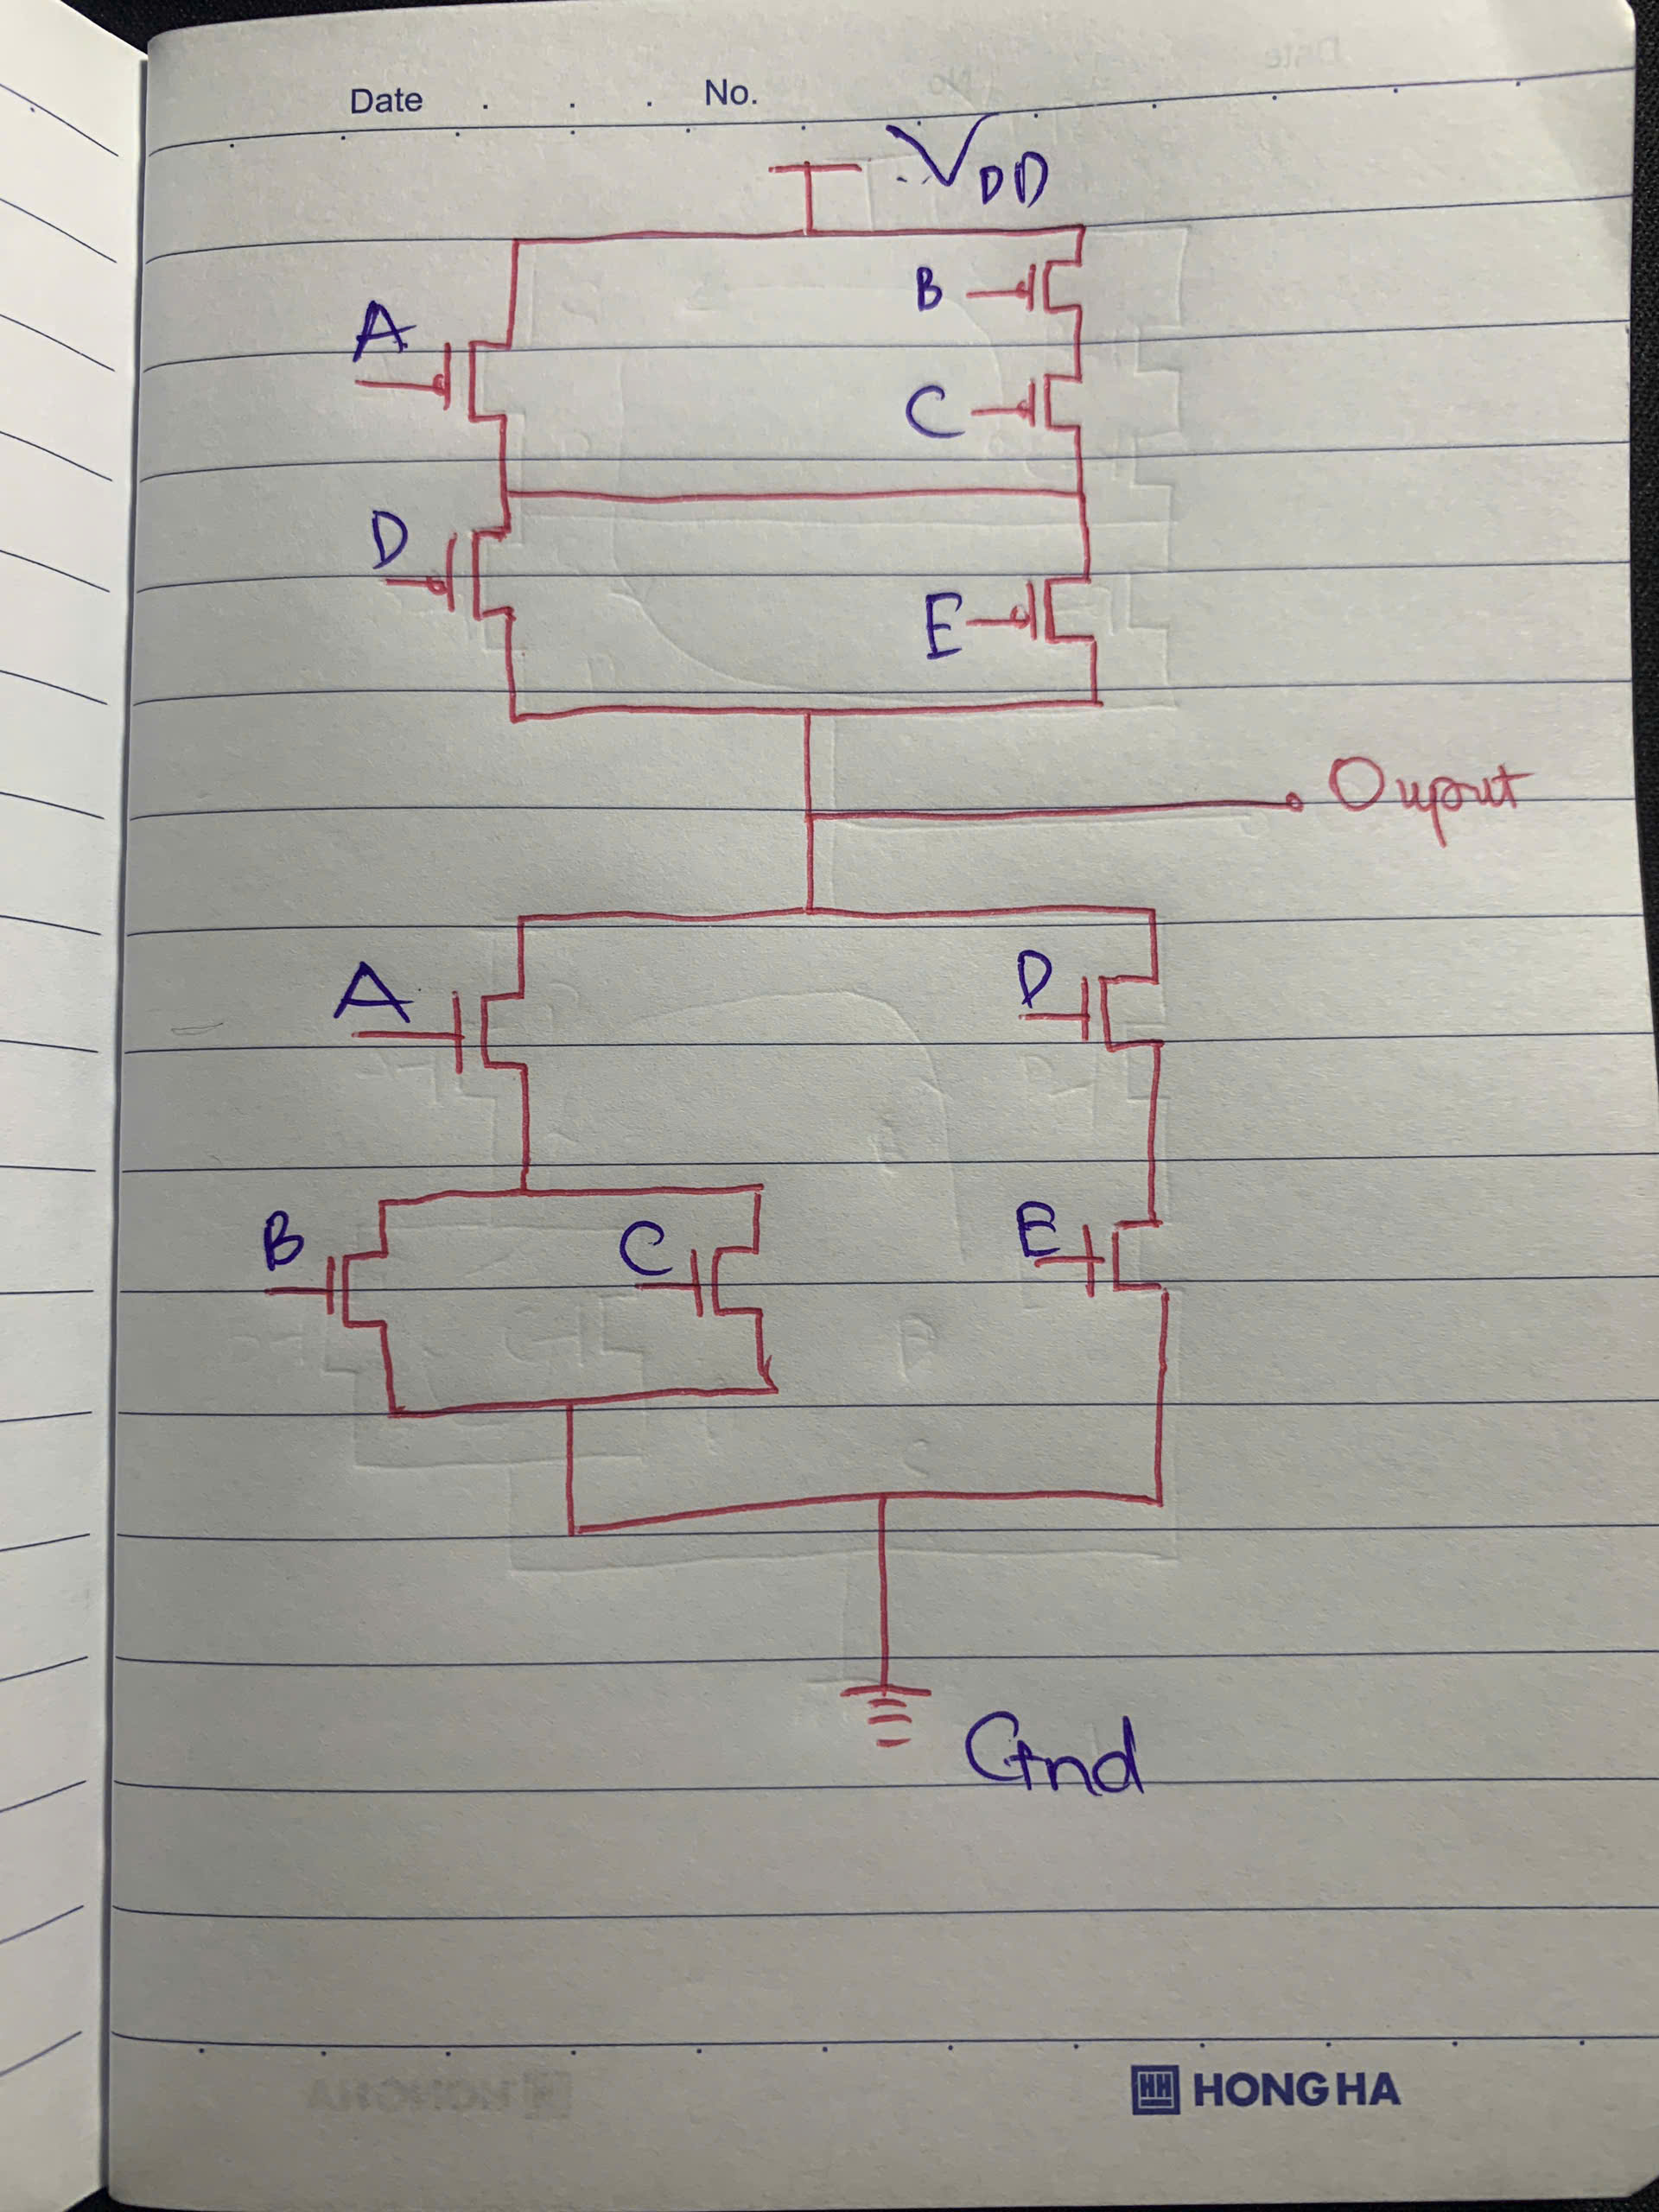
\includegraphics[width=0.5\textwidth]{../PNG/ViDuSchematic.jpg}
    \caption{PMOS và NMOS}
    \label{fig:PMOS_NMOS}
\end{figure}

Tiếp theo, chúng ta cần tìm đường đi Euler của schematic diagram cho cùng NMOS pull-down và PMOS pull-up.

Ở đây, chúng ta sẽ tìm đường đi Euler cho vùng PMOS pull-up đầu tiên và sau đó cho vùng NMOS pull-down sẽ giống với PMOS tìm được.

\begin{figure}[H]
    \centering
    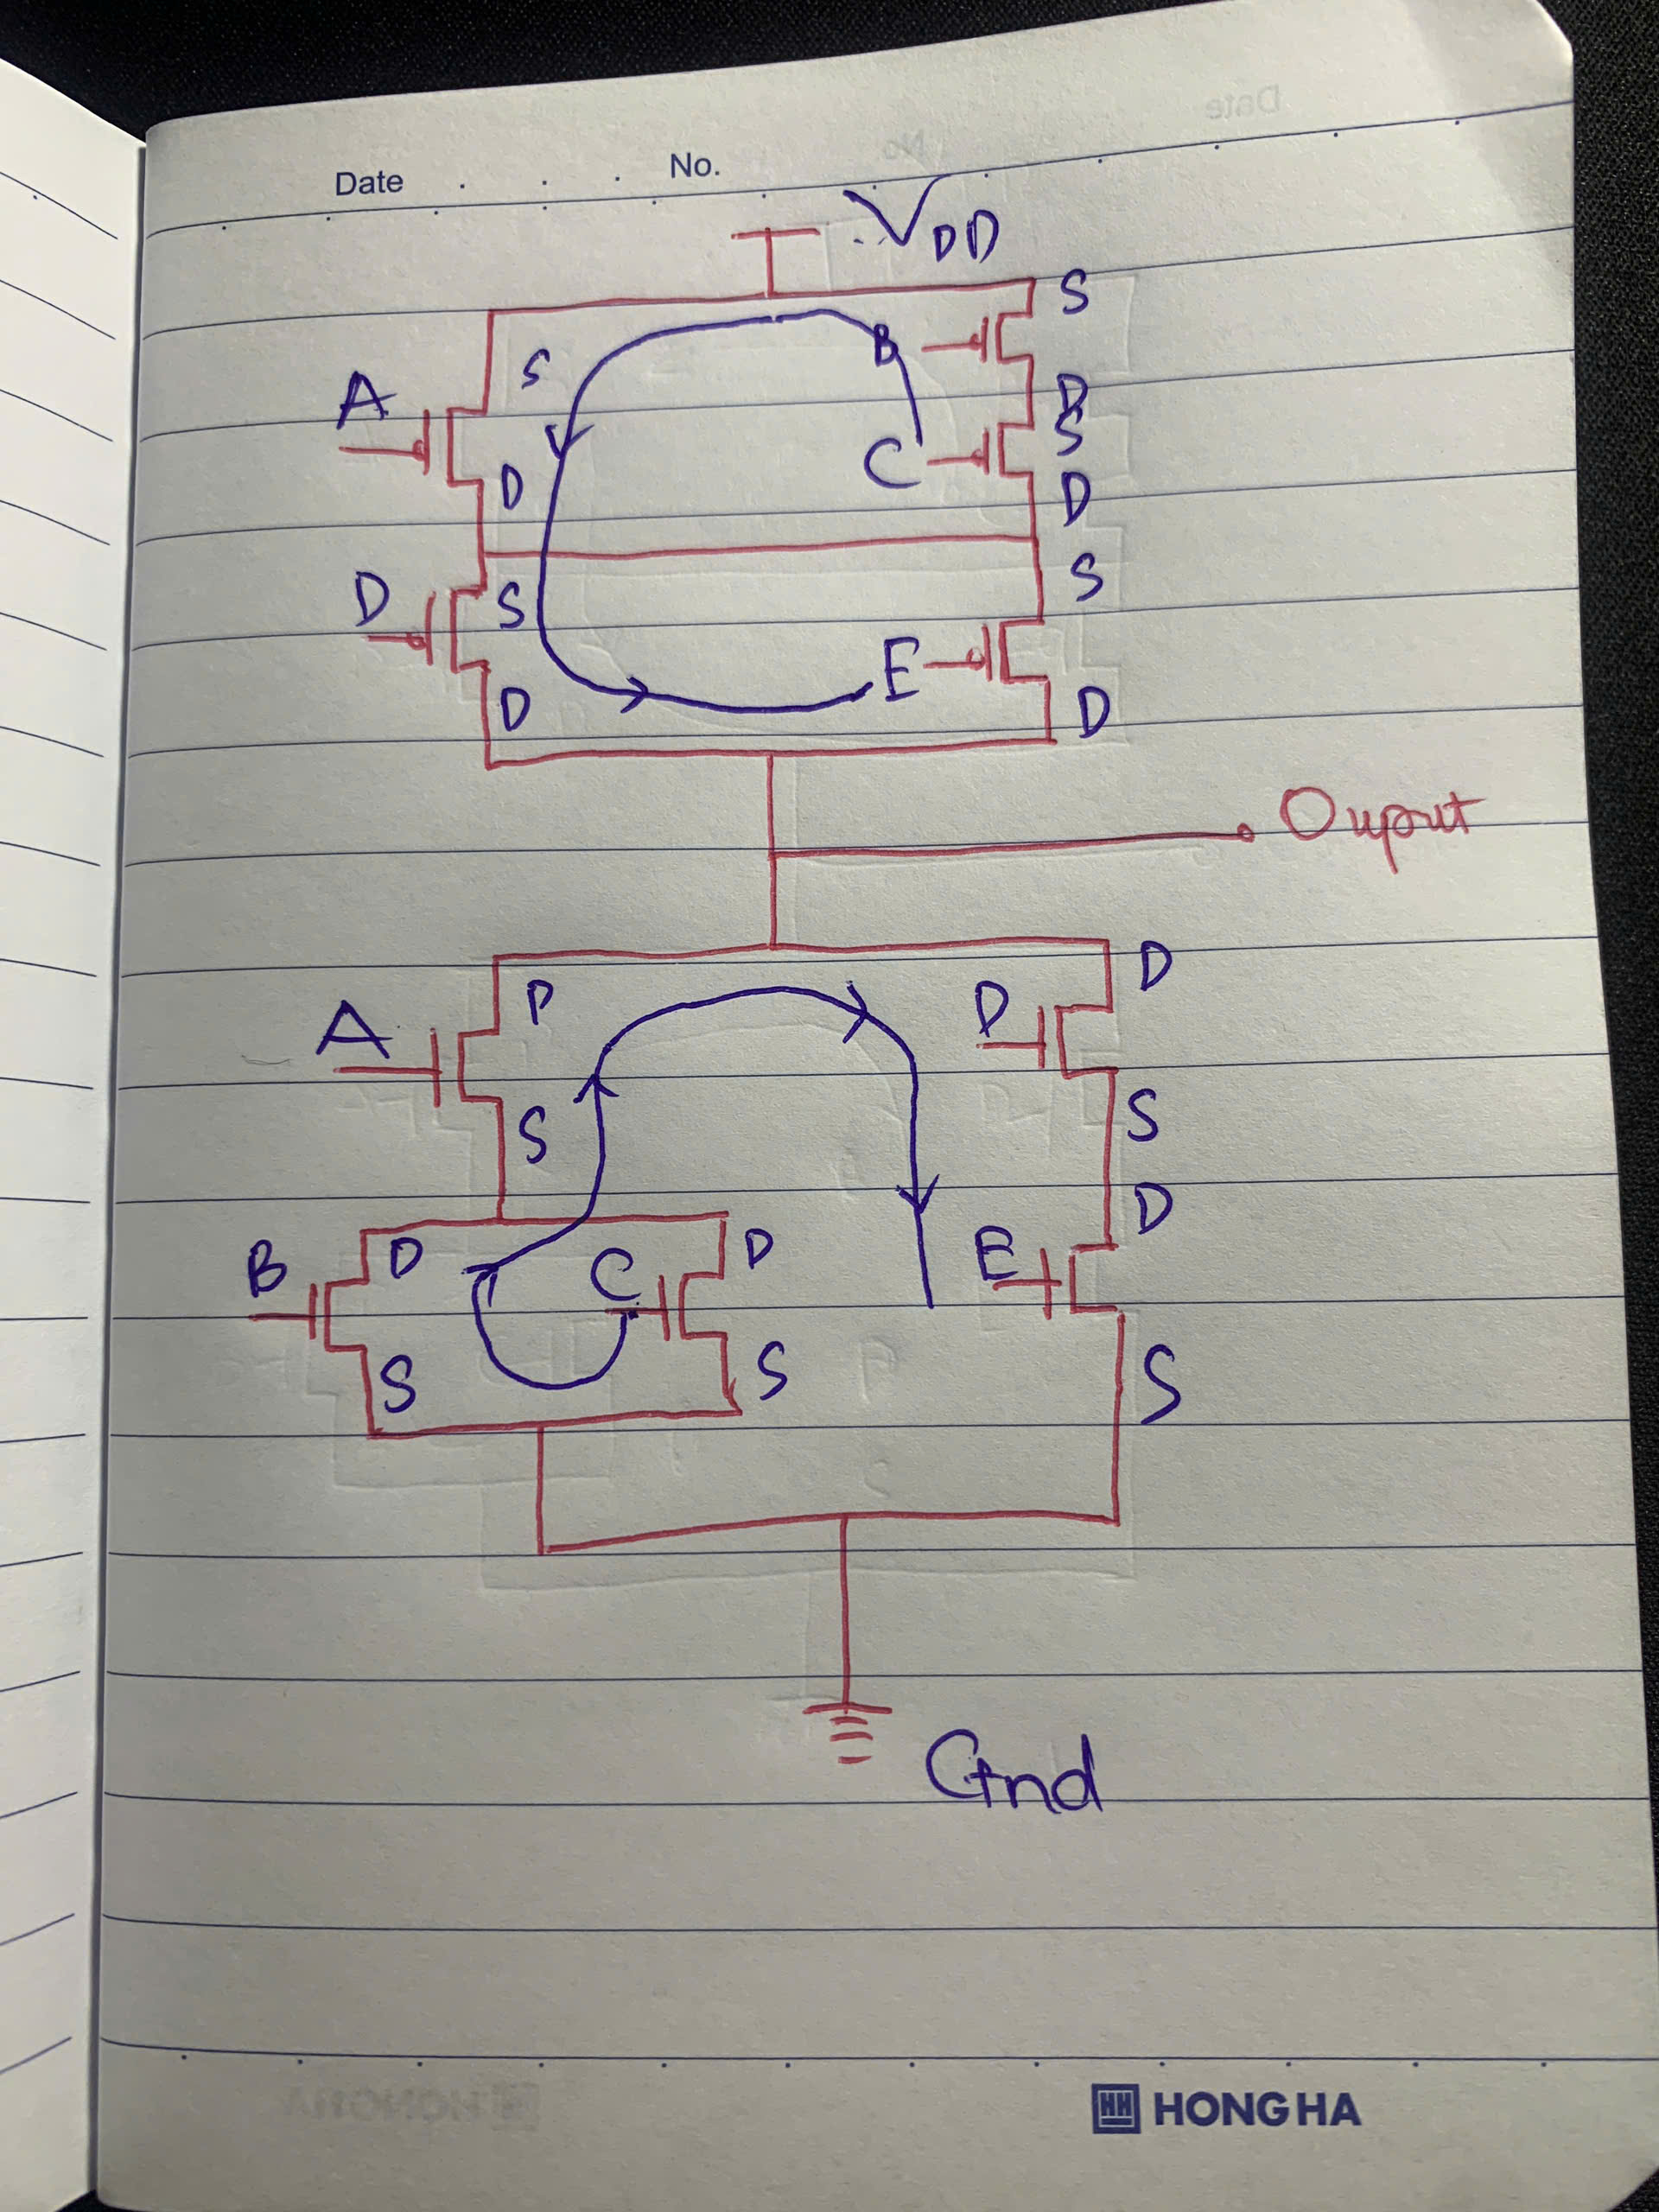
\includegraphics[width=0.5\textwidth]{../PNG/Euler_CMOS.jpg}
    \caption{Đường đi Euler trong CMOS}
    \label{fig:Euler_CMOS}
\end{figure}

\begin{figure}[H]
    \centering
    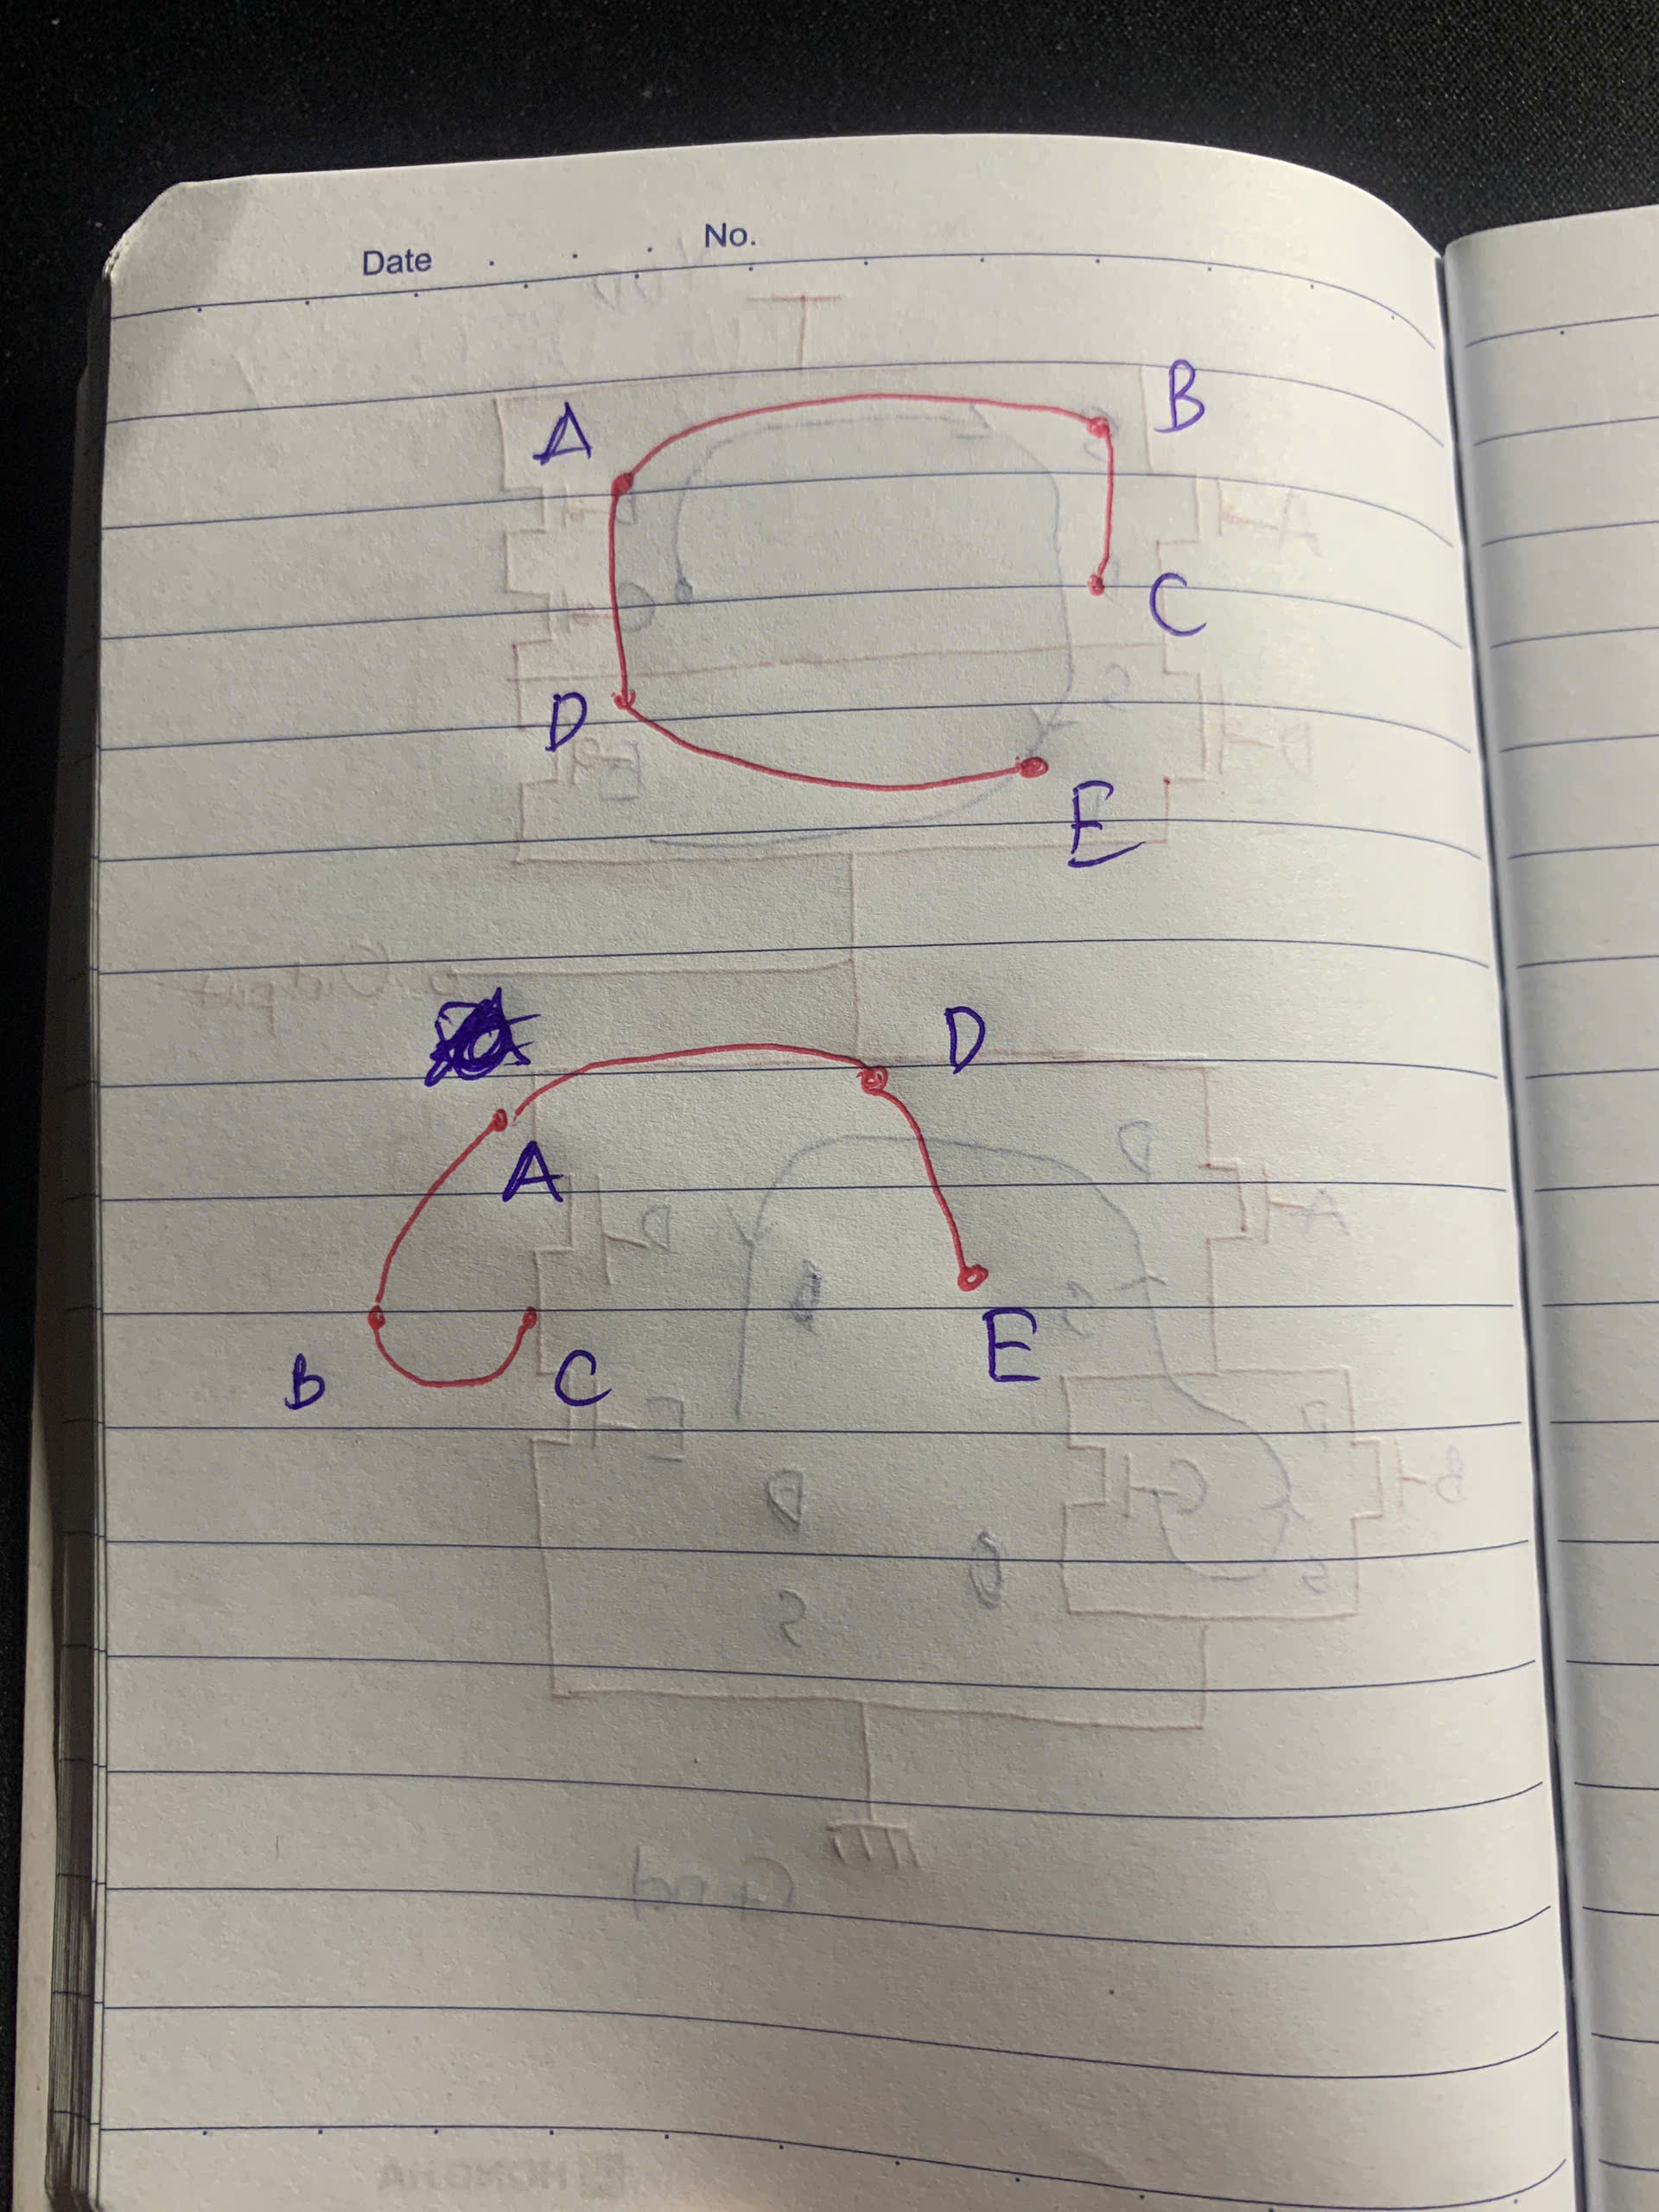
\includegraphics[width=0.4\textwidth]{../PNG/Euler_alone.jpg}
    \caption{Đường Euler khi vẽ riêng}
    \label{fig:Euler}
\end{figure}

Cuối cùng, ta sẽ vẽ Stick Diagram từ đường đi Euler đã tìm được.    

\begin{figure}[H]
    \centering
    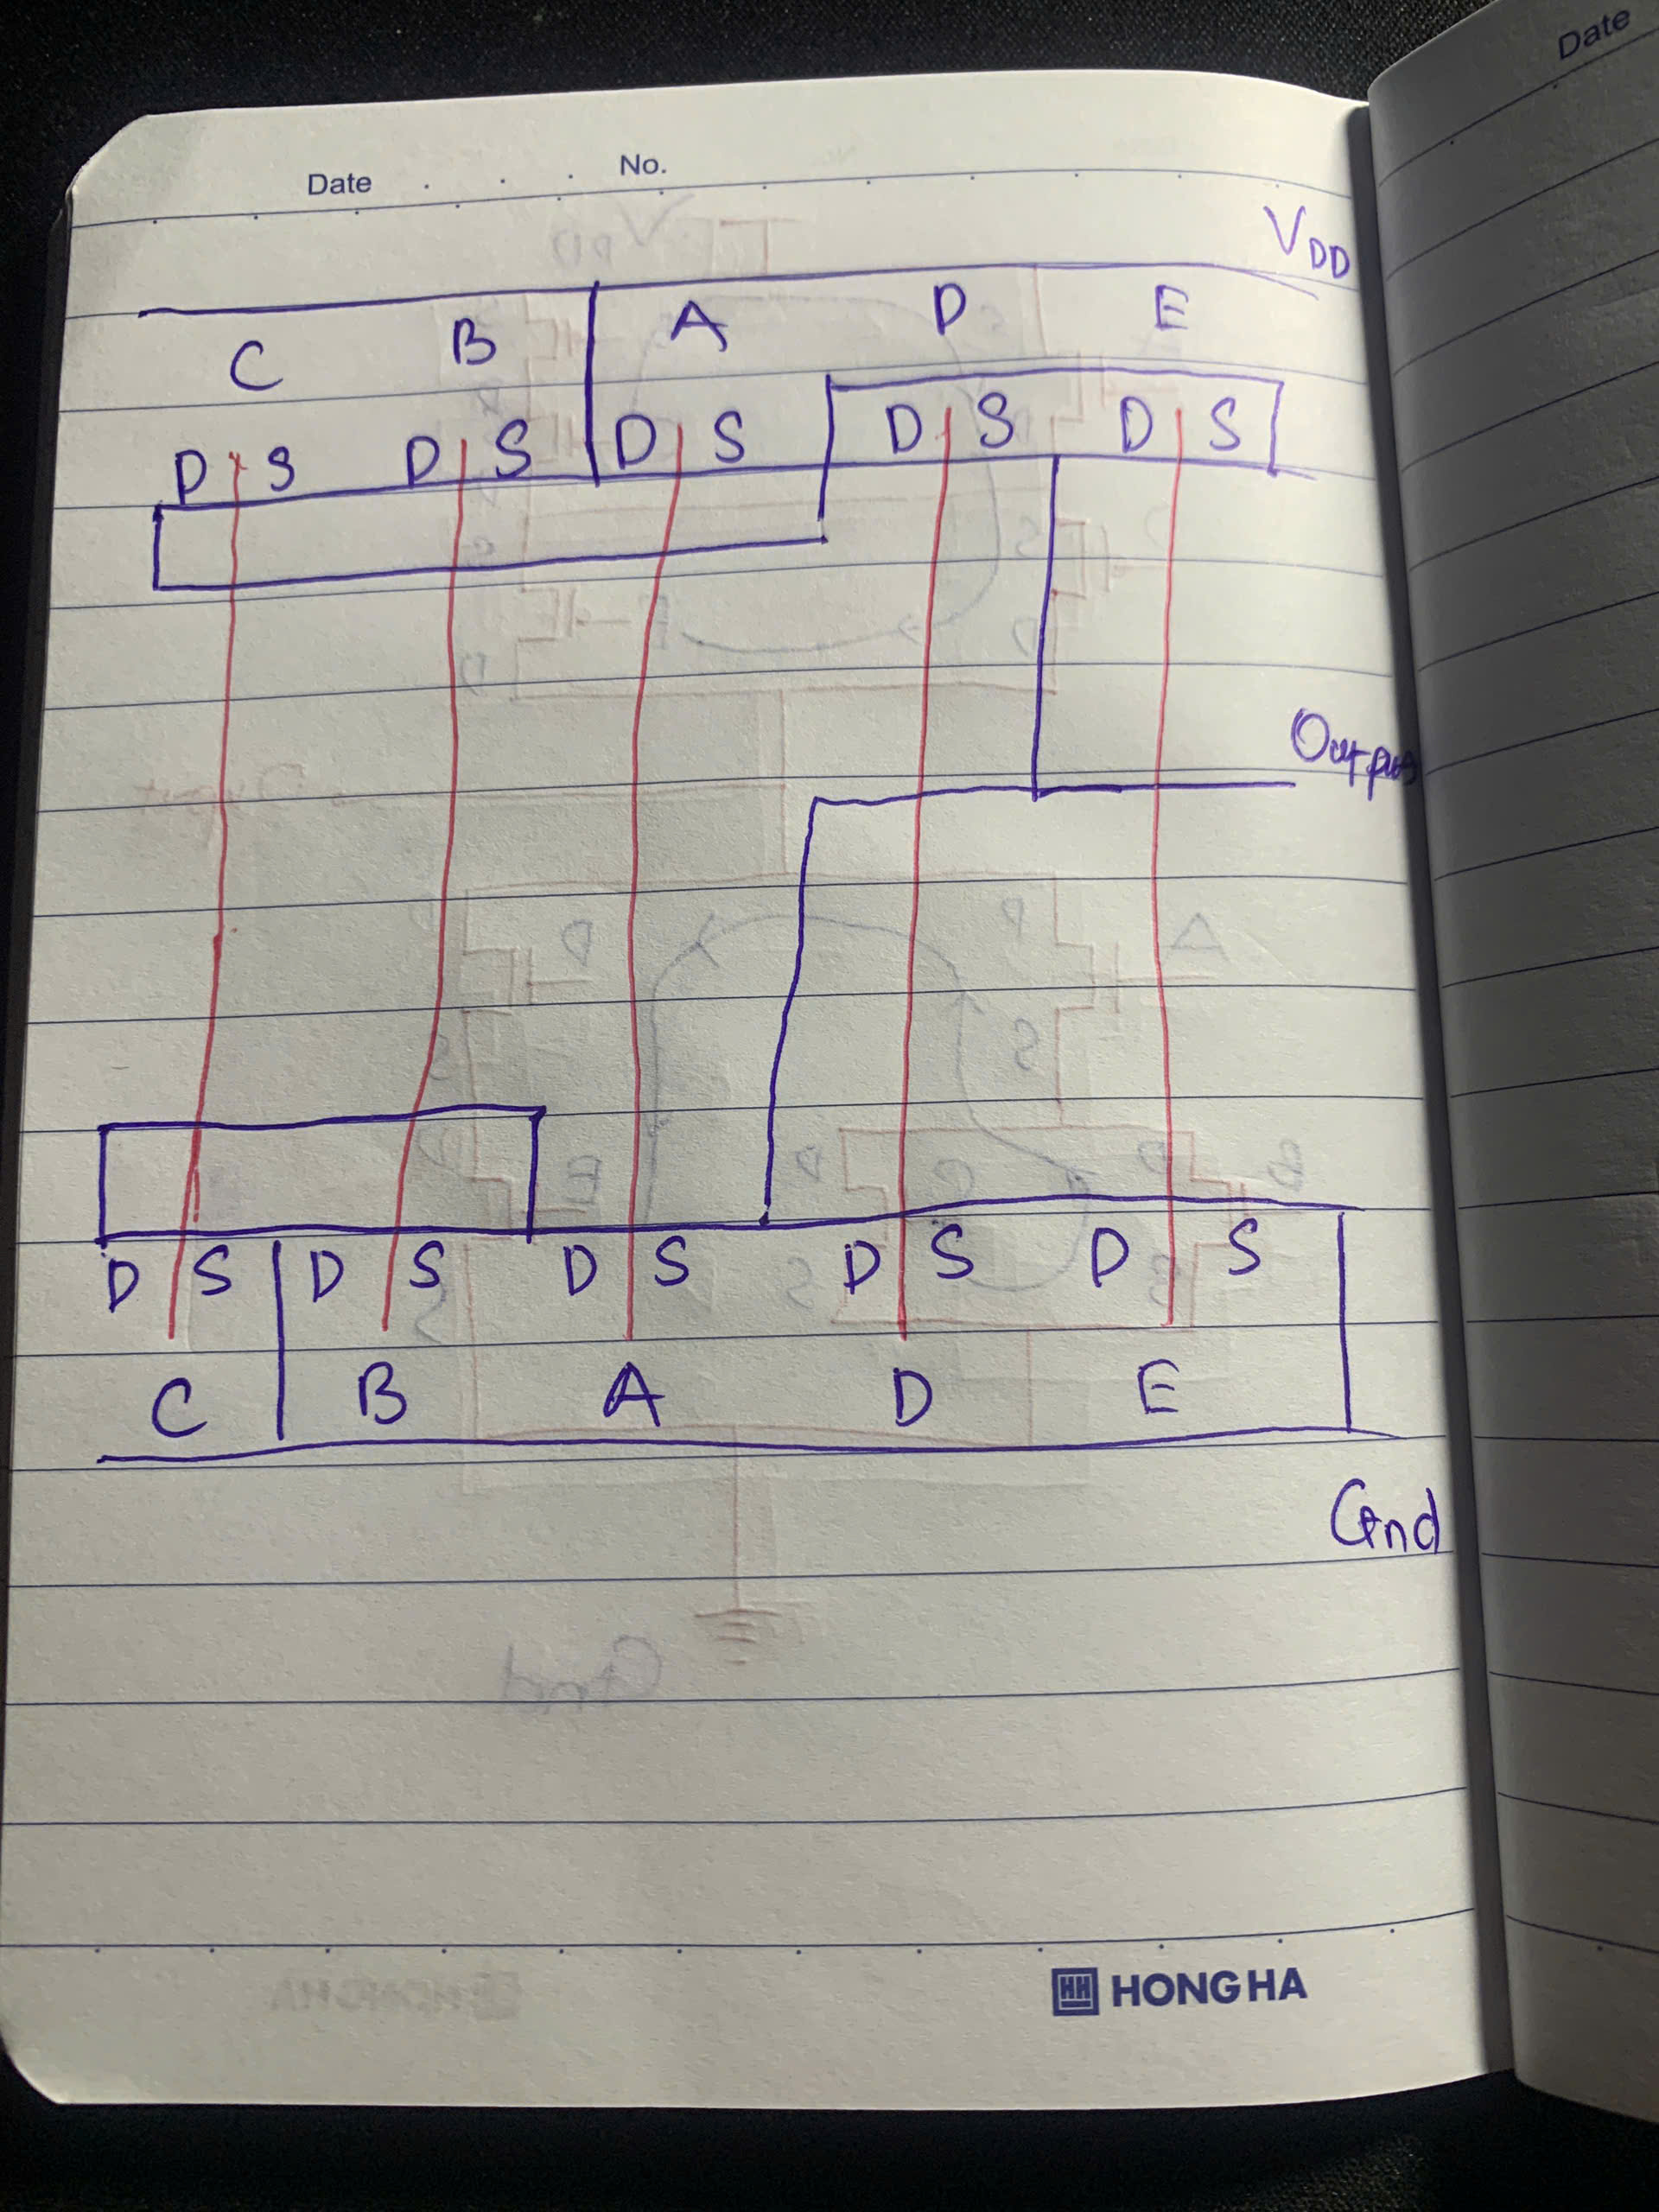
\includegraphics[width=0.8\textwidth]{../PNG/Stick_handwrite.jpg}
    \caption{Stick Diagram}
    \label{fig:Stick_Diagram}
\end{figure}

Như vậy, thuật toán để biểu diễn stick diagram từ biểu thức Boolean là:\\
\textbf{Vẽ schematic diagram -> Tìm đường đi Euler -> Vẽ stick diagram}.
\newpage
%2.
\subsection{Hiện thực bằng Python}
%2.1
\subsubsection{Vẽ Schematic và tìm đường đi Euler trên Python}
Đây là phần khó nhất của bài tập, vì từ một biểu thức Boolean, ta có thể vẽ được rất nhiều trường hợp của stickdiagram.
Nhưng đối với yêu cầu của bài toán, ta phải vẽ được trường hợp của stick diagram của biểu thức Boolean được nhập từ bàn phím
sao cho vùng NMOS pull-down và PMOS pull-up có chung đường đi Euler.
%2.1.1
\paragraph{Hướng tiếp cận}
Không thể vẽ schematic diagram 1 cách trực tiếp từ biểu thức Boolean.
Thay vào đó, ta sẽ sử dụng đồ thị (Graph) để mô hình hóa schematic diagram.

Vì schematic diagram gồm 2 vùng là NMOS pull-down network và PMOS pull-up network, nên ta sẽ tạo 2 đồ thị tương ứng với 2 vùng này, 
với node là các biến đầu vào của Boolean.

Ví dụ: \( Y = \overline{A *(B + C) + D * E} \) thì Node sẽ là:
\textbf{A, B, C, D, E}

Tuy nhiên, để biểu diễn các đường đi trong Schematic Diagram thông qua các cạnh trong 
đồ thị thì các node trên là chưa đủ. Vì ta sẽ không biết là Source hay Drain của CMOS
nối với nhau. Để giải quyết, thì ta sẽ thêm vào các node biểu diễn:
\begin{center}
\textbf{AS, AD, BS, BD, CS, CD, DS, DD, ES, ED}
\end{center}
%2.1.2
\paragraph{Tạo đồ thị mô hình hóa NMOS pull-down network và tìm đường đi Euler}
%a. và b.
\begin{enumerate}[label=\alph*.]
    \item{Tạo đồ thị mô hình hóa NMOS pull-down network}
    \addcontentsline{toc}{subsubsection}{\hspace{7.5em}a. Tạo đồ thị mô hình hóa NMOS pull-down network}\\
%Nội dung 2.1.2.a
Ta phải vẽ 2 đồ thị sao cho chúng có chung giải thuật Euler. Đầu tiên, 
ta sẽ vẽ vùng pull-down trước theo giải thuật sau đây:
    \begin{figure}[H]
        \centering
        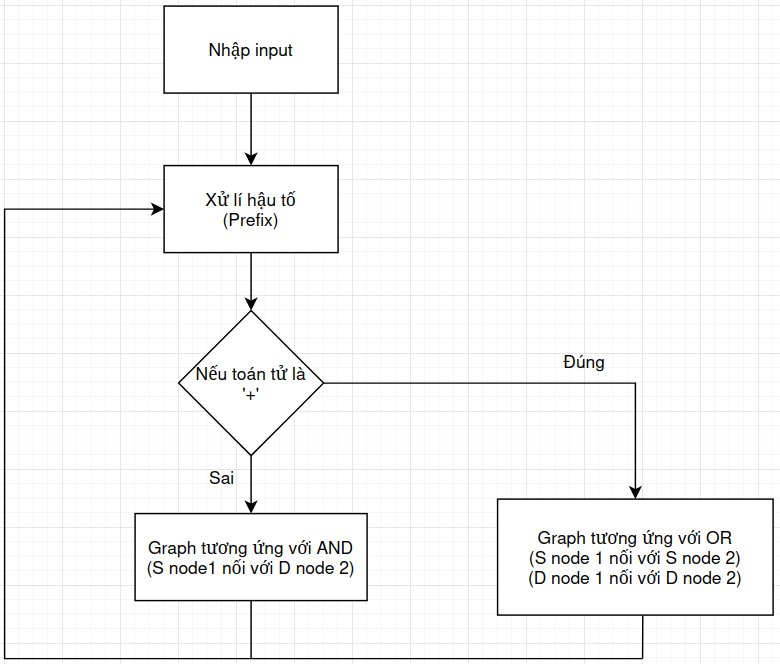
\includegraphics[width=0.8\textwidth]{../PNG/Algorithm_NMOS.png}
        \caption{Thuật toán NMOS}
        \label{fig: NMOSAlgorithms}
    \end{figure}
Việc vẽ đồ thị rất phức tạp, giải thuật trên là tóm gọn và đơn giản nhất của thuật
toán sử dụng trong Python. Ta cần biết rằng để vẽ đồ thị mô hình hóa ghép OR
thì Source và Drain của các node song song với nhau được nối tương ứng: Source-Source,
Drain-Drain.

Khi mô hình hóa phép AND thì sẽ có 2 trường hợp khả thi: Source node 1 - Drain node 2 
hoặc Source node 2 - Drain node. Ta phải quy định sử dụng một trường hợp duy nhất.

Xử lí tính toán biểu thức hậu tố là ta sẽ mô phỏng các phép AND và OR theo quy tắc toán tử hậu tố.

Ví dụ : \(Y = \overline{A *(B + C) + D * E}\) thì sẽ xử lí :\\
1. B + C : Lưu B => node 1, C => node 2. Vẽ đồ thị mô phỏng node 1 OR node 2.\\
2. A * (B + C) : Lưu A => node 1, B + C => node 2.Vẽ đồ thị mô phỏng node 1 AND node 2.\\
3. D * E : D => node 1, E => node 2. Vẽ đồ thị mô phỏng node 1 AND node 2.\\
4. A * (B + C) + D * E : Lưu A * (B + C) => node 1, D * E => node 2.Vẽ đồ thị mô phỏng node 1 OR node 2.
    \item{Tìm đường đi Euler cho vùng NMOS pull-down network}
    \addcontentsline{toc}{subsubsection}{\hspace{7.5em}b. Tìm đường đi Euler cho vùng NMOS pull-down network}\\
Mặc dù thực tế chúng ta sử dụng đường đi Euler nhưng định nghĩa của nó không phù hợp với trong thuật toán.
Vì Euler là đường đi qua hết tất cả các cạnh của đồ thị và chỉ hoạt động đúng khi vẽ schematic diagram,
còn trong đồ thị thì không.

Thay vì sử dụng đường đi Euler, ta sẽ sử dụng đường đi Hamilton thay thế để có thể phù hợp cho cả 2 đồ thị.
Để tránh việc liệt kê thiếu các cạnh trong đồ thị bằng đường đi Hamilton, ta chỉ cần đọc tất cả các cạnh có trong đồ thị
và vẽ Stick Diagram tương ứng với Hamilton tìm được.

Tóm lại, đường đi Euler (đường đi qua tất cả các cạnh trong đồ thị) có thể được
thay thế bằng cách kết hợp đường đi Hamilton (đường đi qua tất cả các điểm trong đồ thị) với việc liệt kê 
tất cả các cạnh của đồ thị.

Thuật toán tìm đường đi Hamilton khá đơn giản, tuy nhiên cần thêm ràng buộc 
là các điểm S và D chung một node luôn được đi chung với nhau. Ví dụ AS-AD, BS-BD,...

Như vậy, với \( Y = \overline{A * (B + C) + D * E} \) thì tacó Euler path (trong Python là Hamilton path)
kết hợp với liệt kê các cạnh trong đồ thị như sau:

\textbf{Euler path NMOS}:[BD, BS, CS, CD, AS, AD, ED, ES, DD, DS]

\textbf{NMOS edge}:[(BS, BD), (BS, CS), (BS, DS), (BD, CD), (BD, AS), (CS, CD),
(CD, AS), (AS, AD), (AD, ED), (DS, DD), (DD, ES), (ES, ED)]
\end{enumerate}
%2.1.3
\paragraph{Tạo đồ thị mô hình hóa PMOS pull-up network và tìm đường đi Euler}
%a. và b.
\begin{enumerate}[label=\alph*.]
    \item{Tạo đồ thị mô hình hóa PMOS pull-down network}
    \addcontentsline{toc}{subsubsection}{\hspace{7.5em}a. Tạo đồ thị mô hình hóa PMOS pull-down network}\\
Đường đi Euler của vùng PMOS pull-up network phải tương tự vùng NMOS pull-down.
Lưu ý rằng chúng ta cần phải tìm Euler path cho vùng PMOS pull-up trước khi tạo
đồ thị cho PMOS pull-up vì khi tạo đồ thị trước sẽ có rất nhiều trường hợp sai lệch.

Ví dụ: A nối tiếp B, ta mong muốn AS - AD - BS - BD.Tuy nhiên, khi tạo đồ thị
bằng thuật toán đã dùng ở NMOS pull-down sẽ có sai lệch : AD - AS - BD - BS. 
Mặc dù trường hợp thứ hai không sai nhưng nó không phải điều ta mong muốn và nó 
có thể dẫn tới việc Euler path ở PMOS pull-up khác với NMOS pull-down

Do đó, ta cần tìm Euler path cho vùng PMOS pull-up trước khi tạo đồ thị. Dựa vào 
Euler path cho vùng NMOS pull-down, ta sẽ dễ dàng tìm được đường đi thích hợp cho PMOS
pull-up bằng cách hoán đổi vị trí S và D của node lẻ trong euler path NMOS.

Ví dụ: \textbf{\( Y = \overline{A *(B + C) + D * E} \)}
\begin{center}
    \textbf{Euler path NMOS: } [BD, BS, CS, CD, AS, AD, ED, ES, DD, DS]\\
    \textbf{B -> C -> A -> E -> D}
\end{center}

Các node lẻ sẽ là C và E. Do đó đường đi Euler thích hợp cho PMOS sẽ là :
\begin{center}
    \textbf{Euler path PMOS: } [BD, BS, CD, CS, AS, AD, ES, ED, DD, DS]\\
    \textbf{B -> C -> A -> E -> D}
\end{center}

Như vậy ta đã tìm được Euler path cho cả 2 đồ thị PMOS và NMOS.
    \item{Tìm đường đi Euler cho vùng PMOS pull-up network}
    \addcontentsline{toc}{subsubsection}{\hspace{7.5em}b. Tìm đường đi Euler cho vùng PMOS pull-up network}

Để tạo đồ thị cho vùng PMOS pull-up network thì ta cần dựa vào Euler path PMOS 
đã tìm được ở mục a. Đồ thị PMOS bắt buộc phải chứa đường đi Euler đã tìm được vì nó 
là đường đi chung cho cả 2 đồ thị. Do đó đầu tiêng ta phải tạo đồ thị ban đầu 
là đường đi Euler trên.

Sau đó, ta sẽ áp dụng phương pháp tạo đồ thị ở mục a để  tạo đồ thị cho vùng 
PMOS pull-up. Tuy nhiên, ta sẽ cần phải kiểm tra thêm việc đã tồn tại sự kết nối
của 2 node chưa vì rất có thể các node và các cạnh đã được hình thành từ việc tạo đồ thị
dựa trên Euler path có sẵn.

Cuối cùng, ta cần chú ý rằng thuật toán áp dụng để tạo đồ thị NMOS pull-down là tạo 
từ 1 đồ thị rỗng ban đầu. Đối với đồ thị PMOS pull-up đã được hình thành dựa trên 
Euler path có sẵn thì thuật toán trên sẽ ít nhiều tạo ra sai lệch và kết quả không mong muốn.

Để giải quyết vấn đề trên, ta sẽ dùng phưong pháp loc và bổ sung dựa trên các cạnh đã tồn tại
ở vùng NMOS pull-down. Ta sẽ liệt kê tất cả các node có thể song song và nối tiếp với nhau trong đồ thị
PMOS từ đồ thị NMOS. Sau đó, ta sẽ so sánh chúng với các node và cạnh trong đồ thị PMOS tạo được. 
Nếu thiếu thì ta sẽ bổ sung thêm vào đồ thị PMOS và nếu sai sẽ loại bỏ chúng khỏi PMOS.

Sơ đồ giải thuật:

Như vậy, với c thì ta sẽ Euler path và đồ thị của vùng PMOS pull-up như sau:

\textbf{Euler path PMOS: } [BD, BS, CD, CS, AS, AD, ES, ED, DD, DS]

\textbf{NMOS edge}:[(BS, BD), (BS, CS), (BS, DS), (BD, CD), (BD, AS), (CS, CD),
(CD, AS), (AS, AD), (AD, ED), (DS, DD), (DD, ES), (ES, ED)]

\end{enumerate}
%2.1.4
\paragraph{Tìm điểm nối nguồn và output}
Bước cuối cùng để mô hình hóa schematic diagram trên Python bằng phương pháp đồ thị 
là tìm các điểm nối nguồn và output. Ta cần tìm các điểm nối nguồn và output trong vùng 
NMOS pull-down và áp dụng giải thuật tương tự cho vùng PMOS pull-up.

Đối với vùng NMOS pull-down network thì các điểm có khả năng nối nguồn là các điểm có hậu tố S 
và ngược lại, các khả năng nối output là các điểm có hậu tố D. Tuy nhiên, không phải tất cả các 
điểm hậu tố S sẽ là các điểm nối với nguồn. Các điểm nối nguồn sẽ là điểm mà ngoài việc nối với node D
của chính nó thì không tồn tại bất kì điểm có hậu tố D nào nối với nó, điều ngược lại cũng đúng
với điểm nối output.

Ví dụ: 

\begin{figure}[H]
    \centering  
    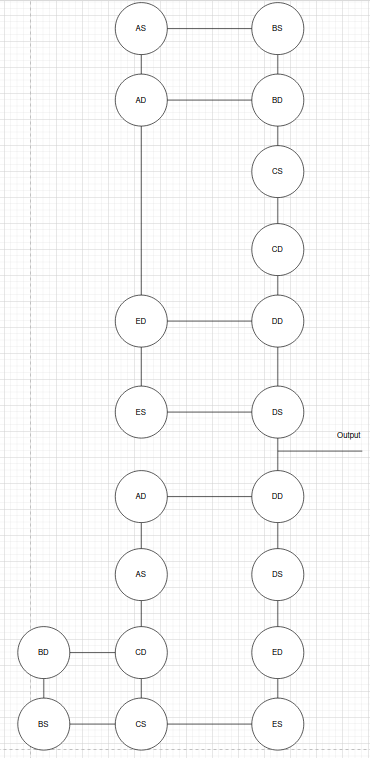
\includegraphics[width=0.5\textwidth]{../PNG/NoiNguon.png}
    \caption{Nối các nguồn}
    \label{fig:ConnectSource}
\end{figure}

• Điểm nối nguồn của NMOS pull-down: BS, CS và DS vì chúng có hậu tố S và không tồn tại điểm
có hậu tố là D kết nối với chúng ngoài chính nó

• Điểm nối output của NMOS pull-down: AD và BD vì chúng có hậu tố D và không tồn tại
điểm có hậu tố là S kết nối với chúng ngòai chính nó.
%2.1.5
\paragraph{Tổng kết mô hình hóa biểu thức Boolean sang Schematic Diagram}
Chương trình sẽ thực hiện lần lượt các bước sau đây để mô hình hóa biểu thức
Boolean sang schematic diagram trên Python:

1. Xử lí tính toán hậu tố đầu vào (NMOS pull-down network).

2. Tạo đồ thị mô hình hóa NMOS pull-down network.

3. Tìm đường đi Euler cho NMOS pull-down network.

4. Tìm đường đi Euler cho PMOS pull-up network.

5. Đảo biểu thức đầu vào và xử lí tính toán hậu tố (PMOS pull-up network)

6. Tạo đồ thị mô hình hóa PMOS pull-up network dựa trên Euler path.

7. Tìm các điểm nối nguồn và đất cho cả 2 đồ thị.

Terminal trong Python hiện kết quả:

\begin{figure}[H]
    \centering  
    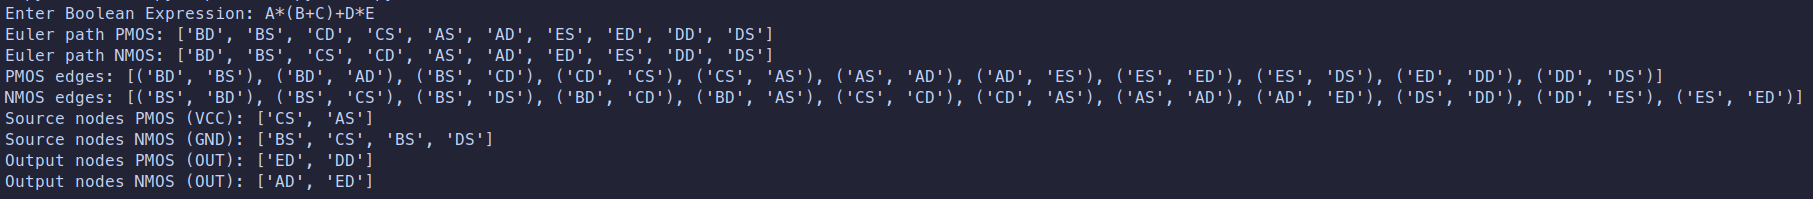
\includegraphics[width=1\textwidth]{../PNG/Terminal_Python.png}
    \caption{Terminal của Python}
    \label{fig:Ter_Py}
\end{figure}
%2.2
\subsubsection{Vẽ Stick Diagram trên Python}
Ta sẽ dùng thư viện matplotlib để vẽ đồ thị.

\paragraph{Vẽ các đường ndiff, pdiff, GND, VDD và các đường đại diện cho các phần tử logic}
\begin{figure}[H]
    \centering  
    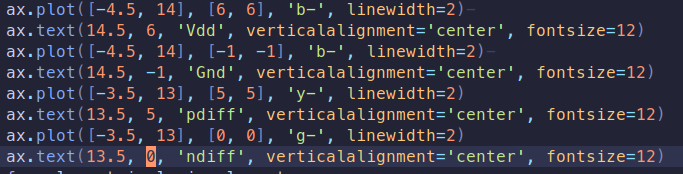
\includegraphics[width=1\textwidth]{../PNG/pdiff_mm.png}
    \caption{PDIFF, NDIFF, GND và VDD}
    \label{fig:PDIFF_MM}
\end{figure}
Trong đoạn code, đường VDD là đường nối 2 điểm có tọa độ (-4.5, 6) và (14, 6),
tương tụ với đừng GND. Đường pdiff là đường nối 2 điểm có tọa độ (-3.5, 5) và (13, 5) với màu vàng
và tương tụ với ndiff là đường màu xanh.

\paragraph{Vẽ đường NMOS, PMOS}

Chạy vòng lặp for để ghi các đỉnh trong mảng ra, mỗi đỉnh cách đều nhau và tất cả cùng nằm trên 
đường thẳng tọa độ y là 5 đối với PMOS (đường pdiff) và đối với NMOS (đường ndiff).

\begin{figure}[H]
    \centering
    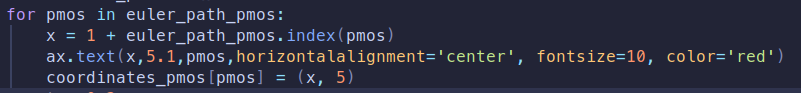
\includegraphics[width=1\textwidth]{../PNG/pmos.png}
    \caption{PMOS}
    \label{fig:pmos}
\end{figure}

\begin{figure}[H]
    \centering
    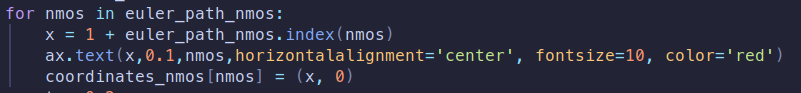
\includegraphics[width=1\textwidth]{../PNG/nmos.png}
    \caption{NMOS}
    \label{fig:nmos}
\end{figure}

Tiếp đến, ta sẽ duyệt qua các cạnh của đồ thị PMOS, dựa vào tọa độ x của từng đỉnh
để vẽ cạnh, vì các đỉnh liền kề nhau đã có sẵn trong Euler path PMOS nên ta chỉ 
xét các đỉnh ở xa nhau (tức khoảng cách lớn hơn 1).

\begin{figure}[H]
    \centering
    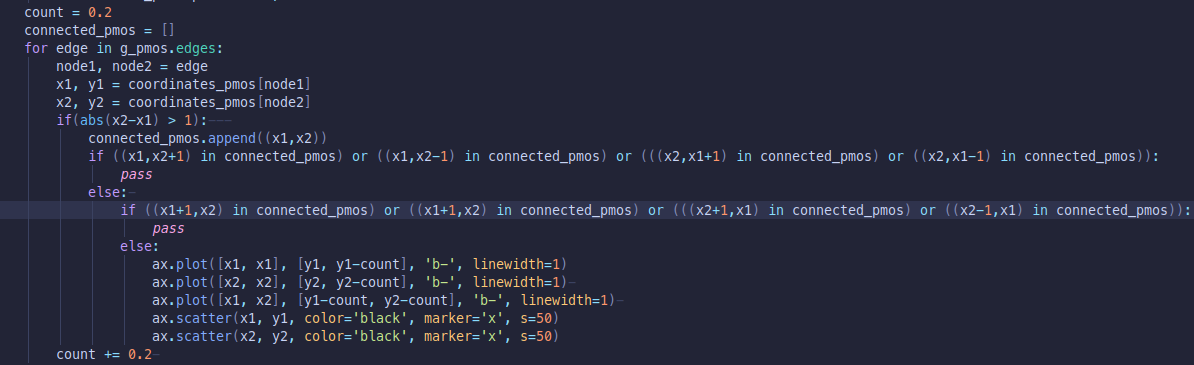
\includegraphics[width=1\textwidth]{../PNG/hehe.png}
    \caption{Duyệt từng đỉnh}
    \label{fig:hehe}
\end{figure}

Trong đoạn code trên, điều kiện kiểm tra để có vẽ cạnh hay không là: đối với đỉnh đầu tiên (x1) thì kiểm tra 
xem đã có kết nối với các đỉnh liền kề với đỉnh thứ hai (x2) hay chưa (x2-1 và x2+1) làm tương tự với đỉnh thứ hai.

Nêú điều kiện đúng thì bỏ qua vẽ cạnh tiếp, nếu sai thì tiếp tục kiểm tra:
đối với đỉnh đầu tiên (x1), kiểm tra xem đã có kết nối giữa các điểm liền kề (x1-1 và x1+1) 
với đỉnh thứ hai (x2) hay chưa, làm tương tụ với đỉnh thứ hai.

Nếu điều kiện kiểm tra lần 2 vẫn sai, thì tiến hành vẽ cạnh. Biến count để điều chỉnh độ cao của các đường nối cho các cặp đỉnh tiếp theo.

Với đồ thị NMOS, thực hiện tương tự.

\paragraph{Vẽ các đường nối nguồn và ngõ ra}

\begin{figure}[H]
    \centering
    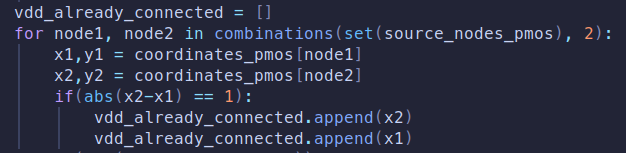
\includegraphics[width=1\textwidth]{../PNG/VDD.png}
    \caption{Vẽ VDD}
    \label{fig:VDD}
\end{figure}

Ta thực hiện việc này vì khi vẽ sẽ ưu tiên các đỉnh liền kề để vẽ duy nhất 1 đường ở giữa 2 đỉnh đó và 
các đỉnh không liền kề sẽ được vẽ theo sơ đồ giải thuật sau:

\begin{figure}[H]
    \centering
    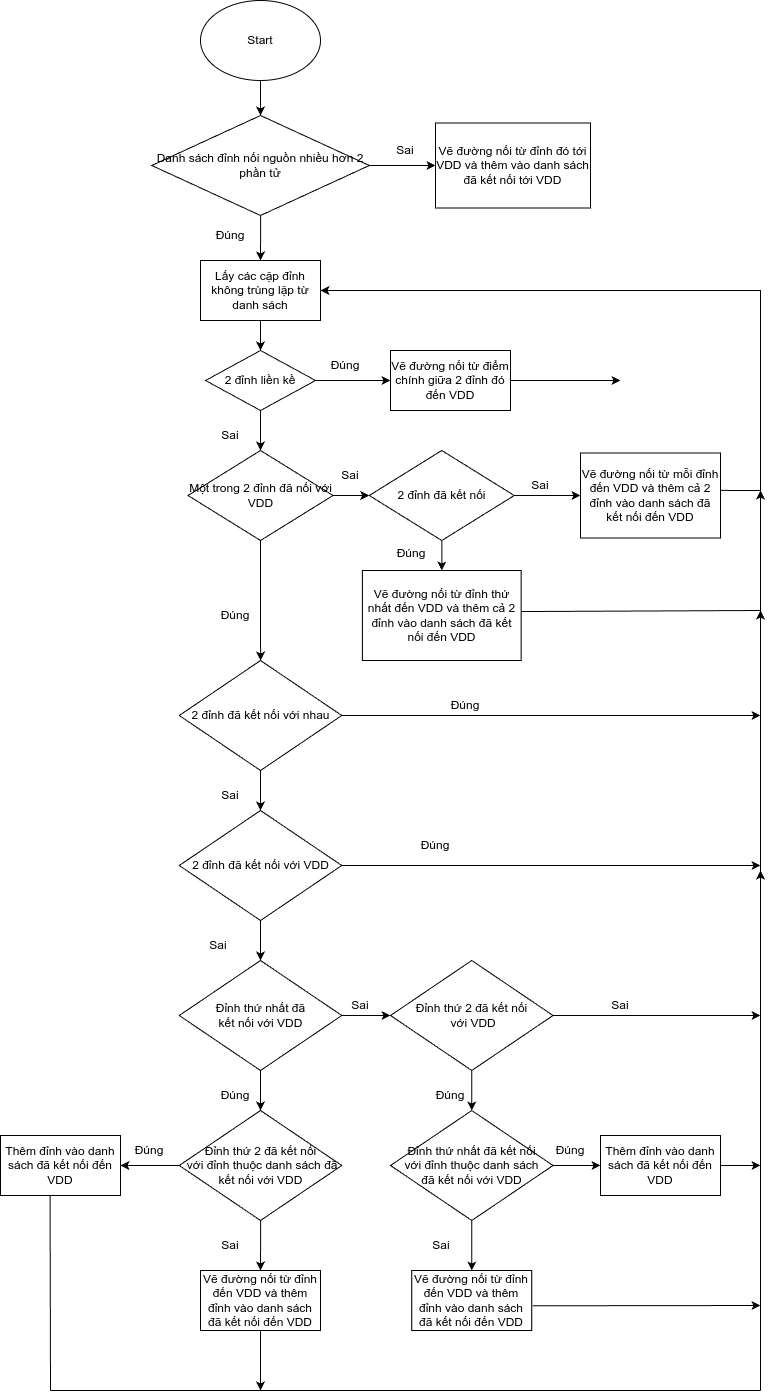
\includegraphics[width=0.7\textwidth]{../PNG/Algorithm_VDD.png}
    \caption{Giải thuật vẽ VDD}
    \label{fig:VDD_Algorithm}
\end{figure}

Đến đây, ta đã hoàn thành xong việc kết nối với VDD, các đường kết nối tới GND, output còn lại đều được vẽ theo cách tương tự như VDD
%3.
\subsection{Kết quả mô phỏng}
Ví dụ về : \( Y = \overline{A *(B + C) + D * E} \)

\begin{figure}[H]
    \centering
    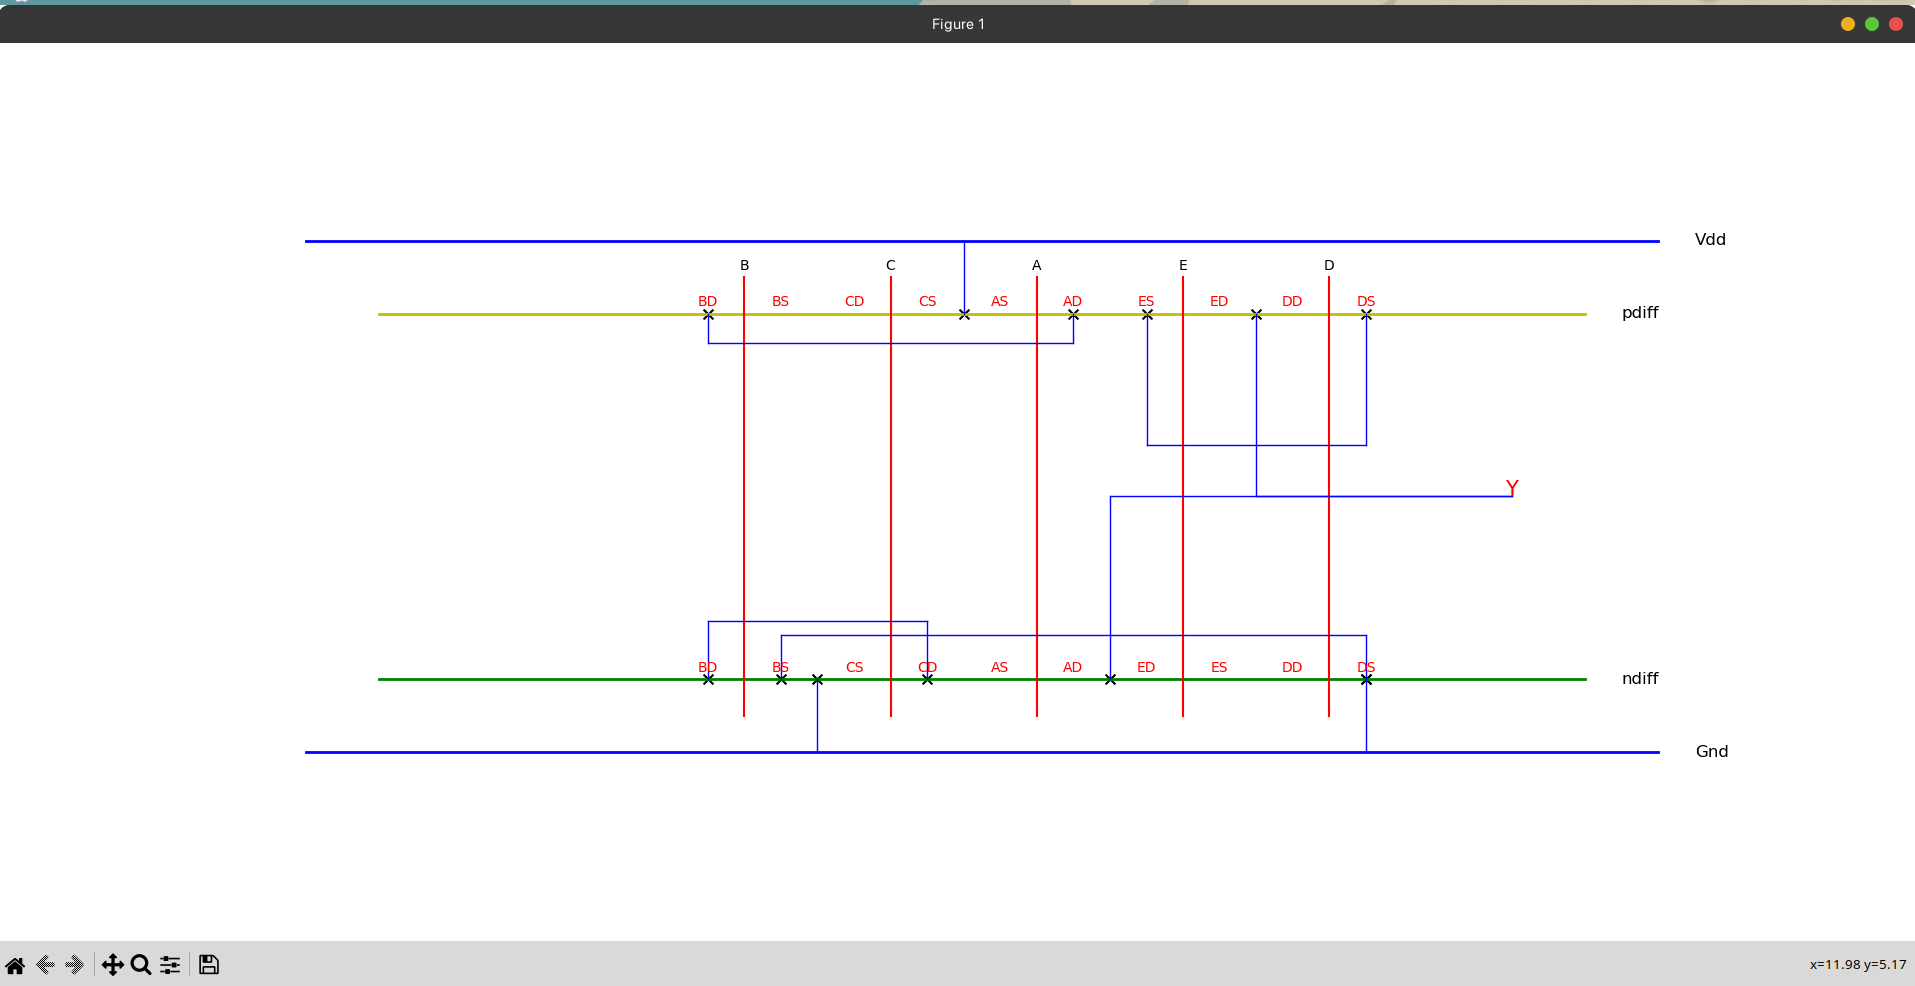
\includegraphics[width=0.8\textwidth]{../PNG/DEMO_Real.png}
    \caption{Demo khi chạy}
    \label{fig:DEMO}
\end{figure}
\newpage
%III.
\section{Tổng kết}
Từ bài tập lớn chuyển đổi biểu thức Boolean thành Stick Diagram, nhóm đã đạt một số yêu cầu sau:

• Biết cách vẽ Stick Diagram của biểu thức Boolean bất kì

• Tìm đường đi Euler cho vùng NMOS, CMOS

• Tìm được điểm nối nguồn và output của từng vùng NMOS, PMOS

• Sử dụng ngôn ngữ C++ và Python để tạo nên Stick Diagram.

Tuy nhiên, chương trình của nhóm vẫn còn cần phải cải thiện ở một số điểm như sau: 

• Chưa có khả năng tối ưu biểu thức đầu vào

• Số lượng phần tử logic quá lớn, có thể dẫn đến sai sót

• Việc vẽ các đường như VDD, GND, ndiff và pdiff chỉ là tương đối (phù hợp cho biểu thức 3-6 biến)
\end{document}